\documentclass[conference]{IEEEtran}
\IEEEoverridecommandlockouts

\usepackage{amsmath,amssymb}
\usepackage{array}
\usepackage{booktabs}
\usepackage{graphicx}
\usepackage[font=footnotesize]{caption}
\usepackage{subcaption}
\usepackage{url}
\usepackage{balance}

\setlength{\textfloatsep}{7pt}
\setlength{\floatsep}{6pt}
\setlength{\intextsep}{6pt}
\setlength{\abovecaptionskip}{4pt}
\setlength{\belowcaptionskip}{0pt}

\title{Immersive 3D Battery Performance and Environmental Intelligence Dashboard Using Raspberry Pi 5 and Ollama}

\author{
\IEEEauthorblockN{Vardhman Mehta}
\IEEEauthorblockA{Enrollment ID: 202201444 \\
\textit{School of Technology, Dhirubhai Ambani University} \\
Gandhinagar, India}
\and
\IEEEauthorblockN{Jaikrit Sanandiya}
\IEEEauthorblockA{Enrollment ID: 202201484 \\
\textit{School of Technology, Dhirubhai Ambani University} \\
Gandhinagar, India}
}

\begin{document}
\maketitle

\begin{abstract}
This project presents a detailed implementation of an immersive WebXR-enabled monitoring platform for battery and environmental intelligence. The system acquires environmental data on a Raspberry Pi 5 using a BME680 sensor, stores and streams the readings safely, and transforms them into a spatial 3D dashboard where users can inspect humidity, temperature, voltage, derived psychrometric behaviour, and geographic location through interactive panels. The frontend is built with React, Vite, Three.js, React Three Fiber, and React Three XR, while environmental visualization is enriched using Recharts, HDRI backgrounds, gradient scene rendering, Mapbox-based geographic context, and panel-level interaction modes such as slider mode, move mode, and experience mode. A local Ollama-based language model complements raw sensor visualization by summarizing the latest environmental condition, threat level, alerts, detailed interpretation, and recommended action in structured JSON form. The result is a monitoring interface that combines IoT data acquisition, immersive visualization, user-centered interaction design, and AI-assisted decision support in a single platform.
\end{abstract}

\begin{IEEEkeywords}
WebXR, Raspberry Pi 5, BME680, React, Three.js, React Three Fiber, sensor dashboard, environmental monitoring, battery monitoring, Mapbox, Socket.IO, Ollama, immersive visualization.
\end{IEEEkeywords}

\section{Introduction}
Conventional monitoring systems usually present readings in the form of tables, line charts, and alert messages on a flat screen. Although such dashboards are useful, they often separate related information into many disconnected widgets. When the user has to monitor environmental conditions, battery-related values, geographic position, and risk interpretation at the same time, a two-dimensional presentation may slow down situational understanding. This is especially important in industrial, mining, logistics, and field-monitoring scenarios where the operator must identify abnormal behaviour quickly and decide what action should be taken.

The present project addresses that problem by building a spatial monitoring dashboard in which data panels are not merely arranged on a page but placed inside a navigable 3D scene. Instead of scrolling through a dense web page, the user can enter the dashboard, focus on specific panels, rearrange them, inspect one panel at a time in slider mode, or stand inside the dashboard in experience mode. In parallel, an analysis subsystem fetches a natural-language environmental report from a backend endpoint and displays status, threat level, alerts, and recommendations.

The application therefore combines four major ideas: real-time sensor monitoring, immersive 3D presentation, contextual location awareness, and AI-assisted interpretation. The same architecture can support a truck, remote battery system, mining support setup, or any mobile asset where environmental conditions and battery behaviour must be tracked together. This report explains the architecture, technologies, data flow, interface design, implementation choices, and all major features in detail.

\section{Problem Statement and Objectives}
The project was designed to solve the problem of fragmented monitoring. In a typical deployment, sensor data is available, but the user still has to mentally combine multiple values before understanding whether the overall condition is safe, drifting, or critical. The project aims to reduce this interpretation burden through a richer interface.

The main objectives of the system are as follows:
\begin{itemize}
\item Build a 3D dashboard that visualizes live environmental and battery-related metrics in an intuitive spatial layout.
\item Integrate historical data, latest readings, and streaming sensor updates into one continuously refreshed frontend.
\item Provide multiple interaction modes so that the same data can be explored casually, analytically, or immersively.
\item Add geographic context through a location-tracing module using Mapbox.
\item Add an LLM-based analysis layer that explains the current state in natural language.
\item Preserve user comfort through background customization, persistent preferences, and focused views for individual panels.
\end{itemize}

\section{System Overview}
At a high level, the application follows a sensor-to-insight pipeline. A Raspberry Pi 5 reads the connected BME680 sensor at fixed intervals, logs readings to a JSONL file, emits live updates through Flask-SocketIO, periodically generates an analysis summary, and exposes the resulting information through web endpoints. The backend exposes historical readings through \texttt{/history}, the most recent reading through \texttt{/data}, a streaming channel through the Socket.IO event \texttt{sensor\_data}, and analysis summaries through \texttt{/analysis}. The frontend consumes these sources, normalizes the values, caches usable history in local storage, and maps the resulting dataset to interactive 3D panels.

The application contains three route-level experiences:
\begin{itemize}
\item \texttt{/home}: a cinematic landing interface that introduces the platform and transitions into the dashboard.
\item \texttt{/dashboard}: the main spatial control room containing all panels, the analysis entry card, background controls, and mode toggles.
\item \texttt{/slider}: a focused reel where one panel is presented at a time for close inspection.
\end{itemize}

Fig.~\ref{fig:overview} shows the main dashboard and the analysis drawer used for LLM-based environmental reporting.

\begin{figure*}[!t]
  \centering
  \begin{subfigure}[t]{0.49\textwidth}
    \centering
    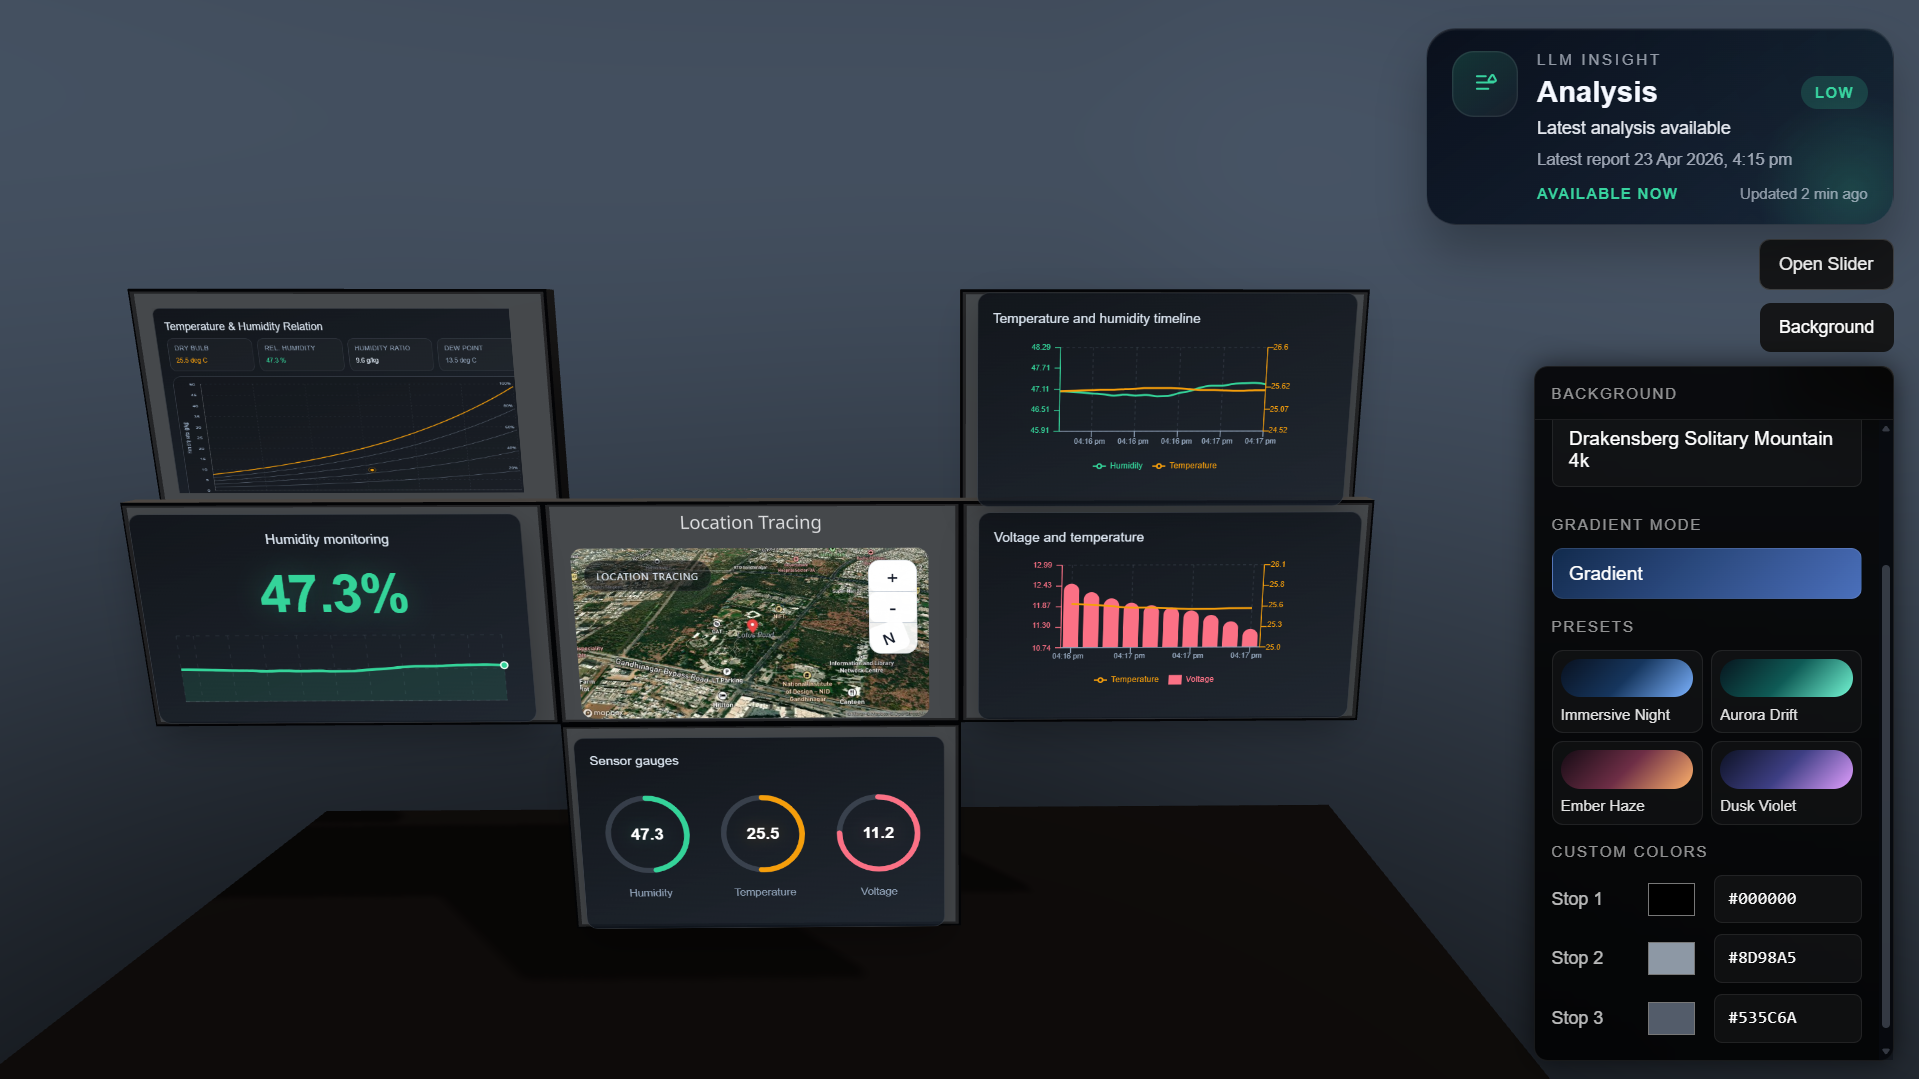
\includegraphics[width=\linewidth]{figures/dashboard-overview.png}
    \caption{Main 3D dashboard containing six monitoring panels and scene controls.}
    \label{fig:dashboard-overview}
  \end{subfigure}
  \hfill
  \begin{subfigure}[t]{0.49\textwidth}
    \centering
    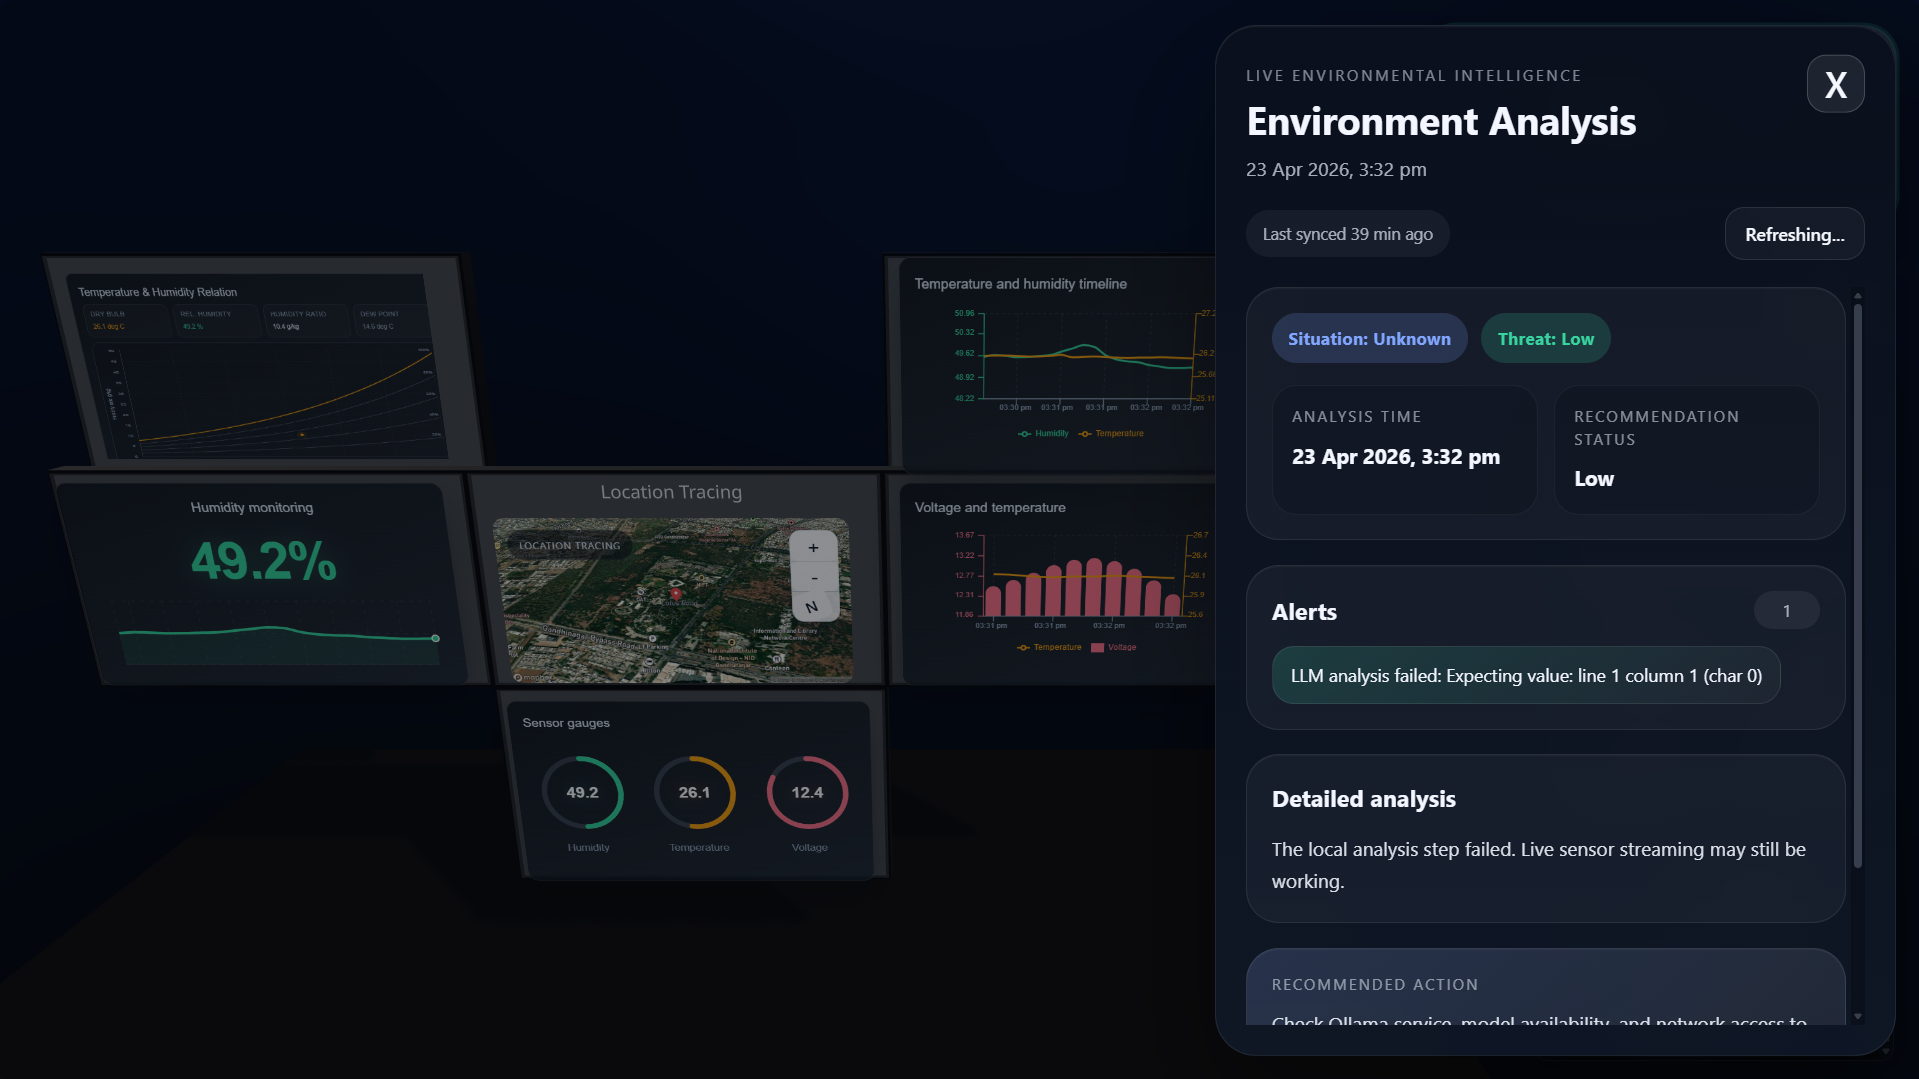
\includegraphics[width=\linewidth]{figures/analysis-panel.png}
    \caption{LLM-based analysis drawer with status, alerts, narrative interpretation, and recommendations.}
    \label{fig:analysis-panel}
  \end{subfigure}
  \caption{Primary interface views of the immersive monitoring system.}
  \label{fig:overview}
\end{figure*}

\section{Software Architecture}
\subsection{Frontend Framework}
The project is implemented as a React application bootstrapped with Vite. React manages component composition, route switching, and state updates, while Vite provides a fast development server and optimized build pipeline. The application uses a route-normalization function in the main application component to switch between the home, dashboard, and slider scenes without needing a heavyweight routing framework.

\subsection{3D Rendering Layer}
The 3D environment is built using Three.js through React Three Fiber. This choice is important because it allows the dashboard to be expressed as React components while still benefiting from the rendering power of Three.js. React Three XR extends this environment to support XR-ready presentation. Orbit controls provide camera navigation in standard desktop mode, while custom camera transitions handle panel focus mode and experience mode.

\subsection{Scene Composition}
The main scene is assembled in the dashboard scene component. It contains:
\begin{itemize}
\item an HDRI or gradient environment for lighting and atmosphere,
\item a stage platform on which the panels are visually anchored,
\item a control room group that instantiates all monitoring panels,
\item optional WebXR session bridging logic,
\item scene-level controls for background settings and navigation actions,
\item the location overlay and the analysis drawer rendered as HTML overlays.
\end{itemize}

\subsection{State and Data Hooks}
The architecture uses focused React hooks so that each subsystem remains modular:
\begin{itemize}
\item \texttt{useChartData}: loads history, listens for live updates, performs fallback polling, and exposes processed sensor values.
\item \texttt{useAnalysisData}: fetches and refreshes LLM analysis snapshots.
\item \texttt{useControlPanels}: maps sensor data to panel definitions and panel content.
\item \texttt{useBackgroundConfig}: reads and persists scene appearance preferences.
\end{itemize}

\subsection{Event-Oriented Coordination}
Some interactions use browser events for loose coupling. For example, the map panel can dispatch an \texttt{open-map} event to show the full-screen location overlay, and other modes can emit \texttt{close-map} when that overlay should disappear. This design avoids deep prop chains and keeps panel components lightweight.

\subsection{Raspberry Pi 5 Backend Services}
The backend is implemented using Flask, Flask-CORS, and Flask-SocketIO in threading mode. Two long-running background tasks are started when the server begins execution: a sensor loop and an analysis loop. The sensor loop reads BME680 measurements every 5 seconds, appends them to \texttt{sensor\_data.jsonl}, updates an in-memory latest-reading object, and emits the reading to connected clients. The analysis loop runs every 5 minutes, reads the most recent 5-minute window of sensor records, computes summary statistics and flags, requests an LLM interpretation, stores the result in \texttt{latest\_analysis.json}, and emits the final analysis object.

\section{Technology Stack}
Table~\ref{tab:stack} summarizes the main technologies used in the project.

\begin{table}[!t]
\caption{Technology Stack Used in the Project}
\label{tab:stack}
\centering
\begin{tabular}{>{\raggedright\arraybackslash}p{1.45cm} >{\raggedright\arraybackslash}p{2.2cm} >{\raggedright\arraybackslash}p{3.55cm}}
\toprule
\textbf{Layer} & \textbf{Technology} & \textbf{Purpose} \\
\midrule
Hardware & Raspberry Pi 5 & Edge device for sensor acquisition, backend hosting, and local inference orchestration \\
Sensor & BME680 & Measures temperature, humidity, pressure, and raw gas resistance \\
Backend API & Flask & Serves REST endpoints for current data, history, and analysis \\
Real-Time Server & Flask-SocketIO & Emits sensor and analysis updates to connected clients \\
Concurrency Safety & FileLock & Prevents read-write corruption while logging and cleaning JSONL data \\
Frontend & React 18 & Component-based UI composition and state-driven rendering \\
Build Tool & Vite & Development server, bundling, and optimized frontend builds \\
3D Engine & Three.js & Core 3D rendering, lighting, audio, and scene objects \\
React--3D Bridge & React Three Fiber & Declarative use of Three.js inside React \\
XR Support & React Three XR & XR session support and immersive presentation integration \\
3D Helpers & Drei & Convenience utilities such as environment support, HTML overlays, and controls \\
Charting & Recharts & Time-series, composed charts, gauges, legends, and tooltips \\
Map Layer & Mapbox GL and React Map GL & Static preview maps and full-screen interactive location overlay \\
Real-Time Data & Socket.IO Client & Live sensor update subscription on the frontend \\
Animation & GSAP & Smooth audio fade-in and fade-out transitions \\
Persistence & Local Storage & Caching sensor history and saving background preferences \\
AI Layer & Ollama with Qwen2.5 0.5B & Local natural-language environmental interpretation and recommendations \\
\bottomrule
\end{tabular}
\end{table}

\section{Data Acquisition and Processing Pipeline}
\subsection{Raspberry Pi 5 and BME680 Sensor Configuration}
The data collection node is built around a Raspberry Pi 5 connected to a BME680 environmental sensor over I\textsuperscript{2}C. The backend configures oversampling for humidity, pressure, and temperature, enables the gas measurement path, and sets the gas heater temperature and duration before beginning continuous monitoring. Each reading contains a timestamp, temperature, pressure, humidity, and raw gas resistance value.

Gas resistance is stored only when the heater state is stable. This is a practical detail that improves data reliability because unstable gas-heater states are not treated as valid air-quality-related samples.

\subsection{Sensor Endpoints}
The frontend is configured to contact a sensor backend using a base URL that can be supplied through \texttt{VITE\_SENSOR\_API\_BASE\_URL}. The code is designed around four backend interfaces:
\begin{itemize}
\item \texttt{/history}: returns a list of previously collected sensor readings,
\item \texttt{/data}: returns the latest reading,
\item \texttt{/analysis}: returns the latest environmental analysis snapshot,
\item \texttt{sensor\_data}: a Socket.IO event that streams new readings in real time,
\item \texttt{analysis\_update}: a Socket.IO event emitted whenever the backend completes a new analysis cycle.
\end{itemize}

\subsection{Normalization}
Incoming readings are normalized before being visualized. The frontend ensures a usable timestamp, converts values to numbers, clamps temperature and humidity to reasonable limits, and rounds values for presentation stability. The normalized structure stores temperature, humidity, pressure, gas resistance, voltage, timestamps, and ordering metadata. This normalization layer decouples the dashboard from raw backend payload irregularities and keeps the charts stable even when individual records are incomplete. In the current version, humidity, temperature, voltage, and location are emphasized visually in the main 3D dashboard, while pressure and gas resistance contribute mainly to backend summarization and LLM analysis.

\subsection{Historical Cache and Fallback Logic}
The \texttt{useChartData} hook improves reliability in three ways:
\begin{itemize}
\item It first attempts to load historical data from the backend.
\item It stores a snapshot of that history in local storage so that a reload does not begin from an empty screen.
\item If the Socket.IO stream is disconnected or unavailable, it periodically polls the latest reading to keep the dashboard active.
\end{itemize}

This hybrid model is useful because immersive dashboards feel broken if the scene remains static after startup. By combining history, live stream, and polling fallback, the interface can remain responsive under imperfect network conditions.

\subsection{Safe Logging and Retention Strategy}
The Raspberry Pi backend stores sensor data in newline-delimited JSON format inside \texttt{sensor\_data.jsonl}. A file lock is used whenever records are read, appended, or rewritten, which reduces the risk of corruption when multiple background operations overlap. A cleanup task runs every 300 seconds and removes records older than 12 hours. This approach keeps the log lightweight enough for edge execution while still preserving a meaningful recent window for analysis and dashboard history.

\subsection{Voltage Handling in the Current Prototype}
One important implementation detail is that the temperature and humidity values are consumed from incoming sensor data, whereas the voltage stream is presently synthesized on the frontend using a bounded sinusoidal signal. This allows the voltage-related panels to remain functional during interface development and interaction testing even when a direct battery voltage feed is not yet integrated. The report therefore treats the voltage panel as a working prototype visualization with a clear path for replacement by real hardware data.

\section{Monitoring Panels and Visual Analytics}
The dashboard is centered around six spatial panels. Each panel serves a different analytical purpose, allowing the user to move from raw values to trends, cross-metric relationships, and contextual interpretation.

\subsection{Psychrometric Relation Panel}
The temperature-humidity relation panel is one of the most technically rich modules. It acts as a psychrometric-style plot that relates dry bulb temperature to humidity ratio and highlights the current operating point with respect to relative humidity curves.

The panel computes saturation vapour pressure according to
\begin{equation}
P_{ws}(T)=0.61078 \exp \left( \frac{17.2694T}{T+237.3} \right),
\end{equation}
where \(T\) is dry bulb temperature in degrees Celsius and \(P_{ws}\) is in kPa.

Humidity ratio is then derived as
\begin{equation}
W = \frac{0.62198 \phi P_{ws}}{P_{atm}-\phi P_{ws}} \times 1000,
\end{equation}
where \(\phi\) is relative humidity as a fraction and \(P_{atm}=101.325\) kPa. The dew point is calculated using a logarithmic approximation:
\begin{equation}
\alpha = \ln(\phi) + \frac{17.625T}{243.04+T}, \qquad
T_{dp} = \frac{243.04\alpha}{17.625-\alpha}.
\end{equation}

This panel therefore goes beyond simple plotting by deriving secondary environmental indicators. It helps the operator understand whether the current combination of temperature and humidity is drifting toward an uncomfortable or risky zone rather than merely seeing those values separately.

\begin{figure}[!t]
  \centering
  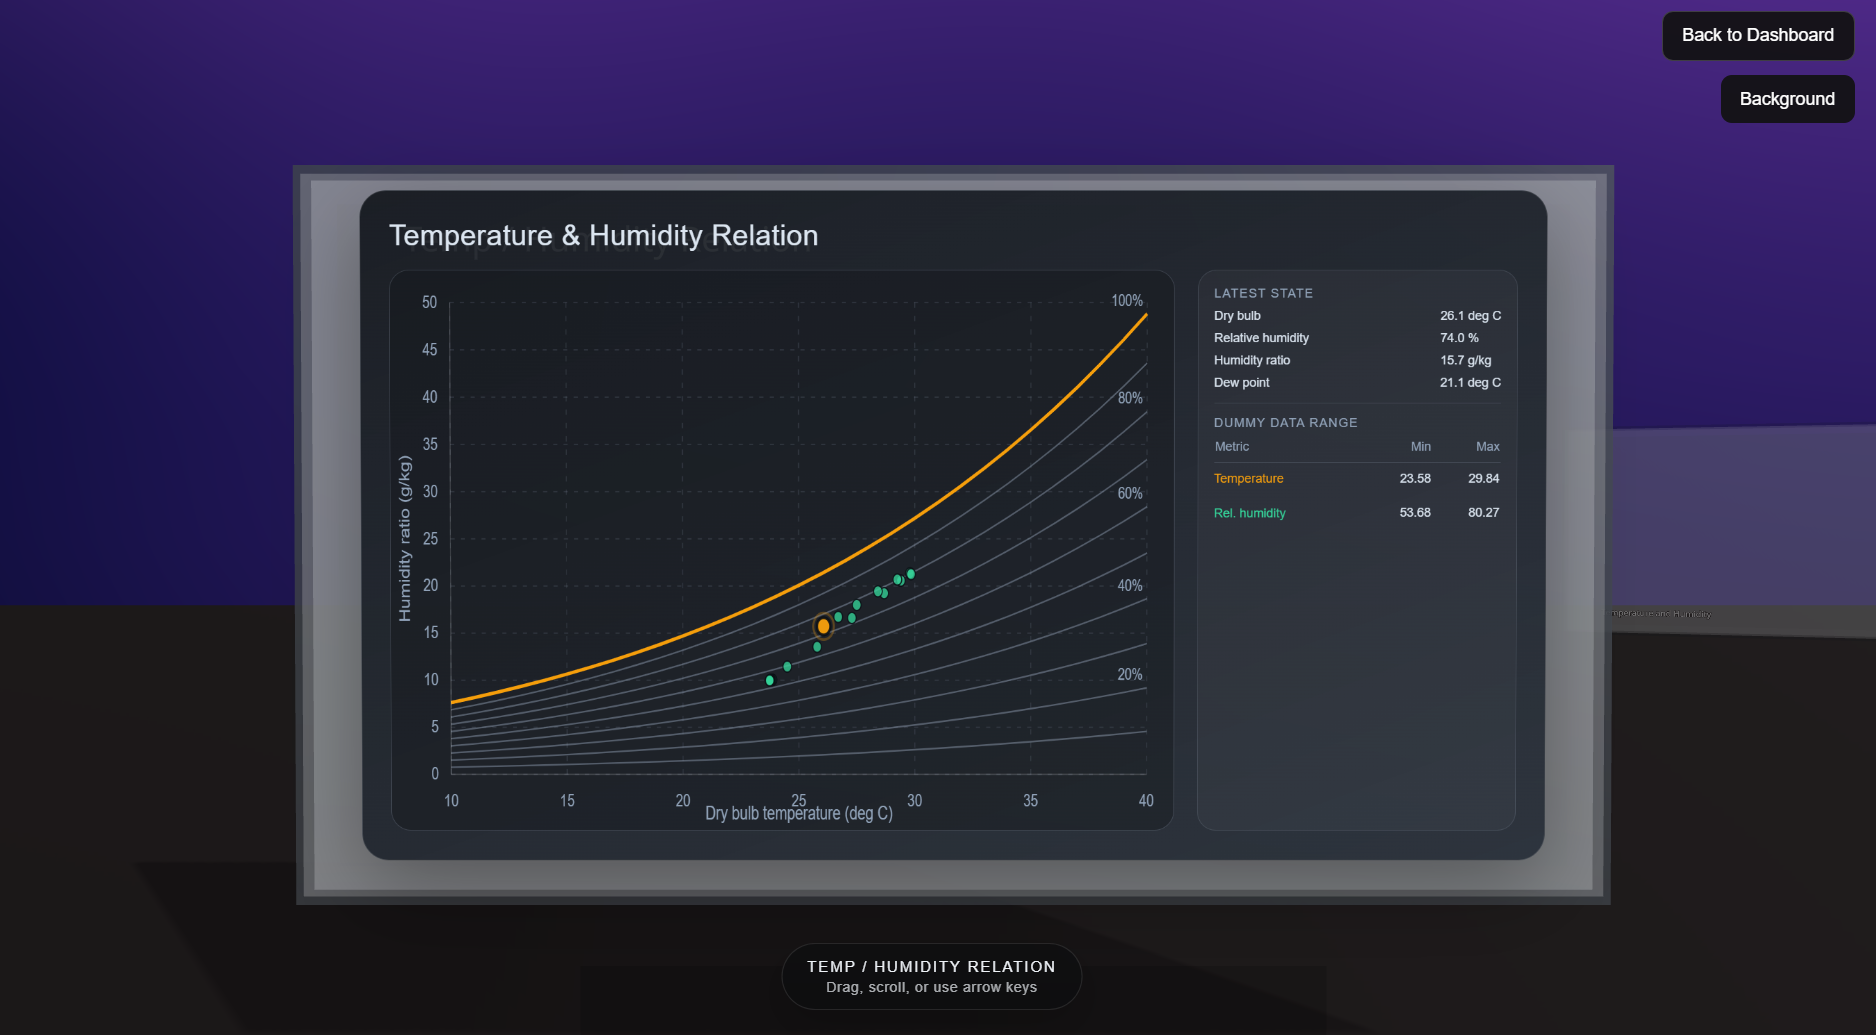
\includegraphics[width=\linewidth]{figures/psychrometric-chart.png}
  \caption{Focused psychrometric-style relation panel showing dry bulb temperature, humidity ratio, and the recent operating trajectory.}
  \label{fig:psychrometric}
\end{figure}

\subsection{Humidity Monitoring Panel}
The humidity monitoring panel presents the current humidity as a large dominant value with a compact trend graph below it. This panel is designed for fast scanning. The numeric emphasis allows an operator to recognize the current state instantly, while the area chart provides short-term trend awareness without demanding extended interpretation.

\begin{figure}[!t]
  \centering
  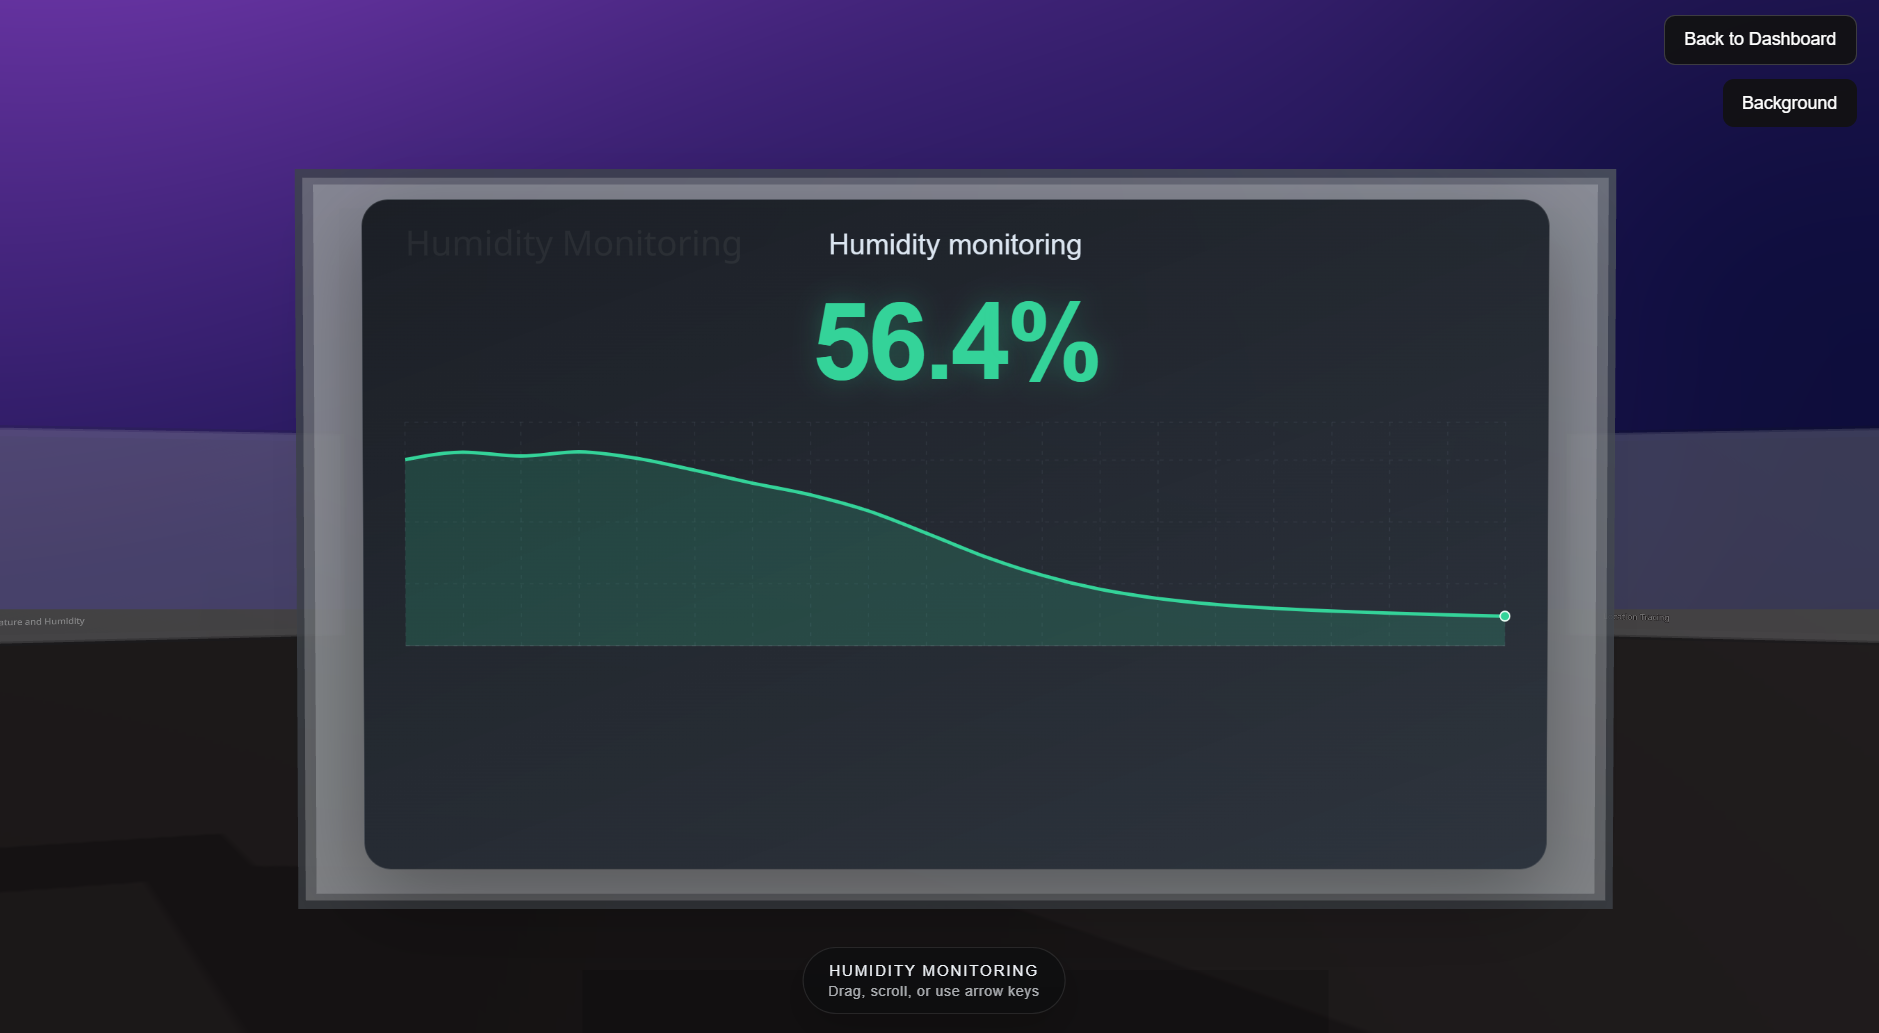
\includegraphics[width=\linewidth]{figures/humidity-monitoring.png}
  \caption{Humidity panel in slider mode, emphasizing the latest value and recent trend.}
  \label{fig:humidity}
\end{figure}

\subsection{Sensor Gauges Panel}
The gauge panel aggregates humidity, temperature, and voltage into circular gauges. This is a compact overview panel intended for quick health checks. The three gauges enable simultaneous reading of the principal metrics without switching attention between independent panels. It is particularly useful when the user wants a short summary before studying the detailed graphs.

\begin{figure}[!t]
  \centering
  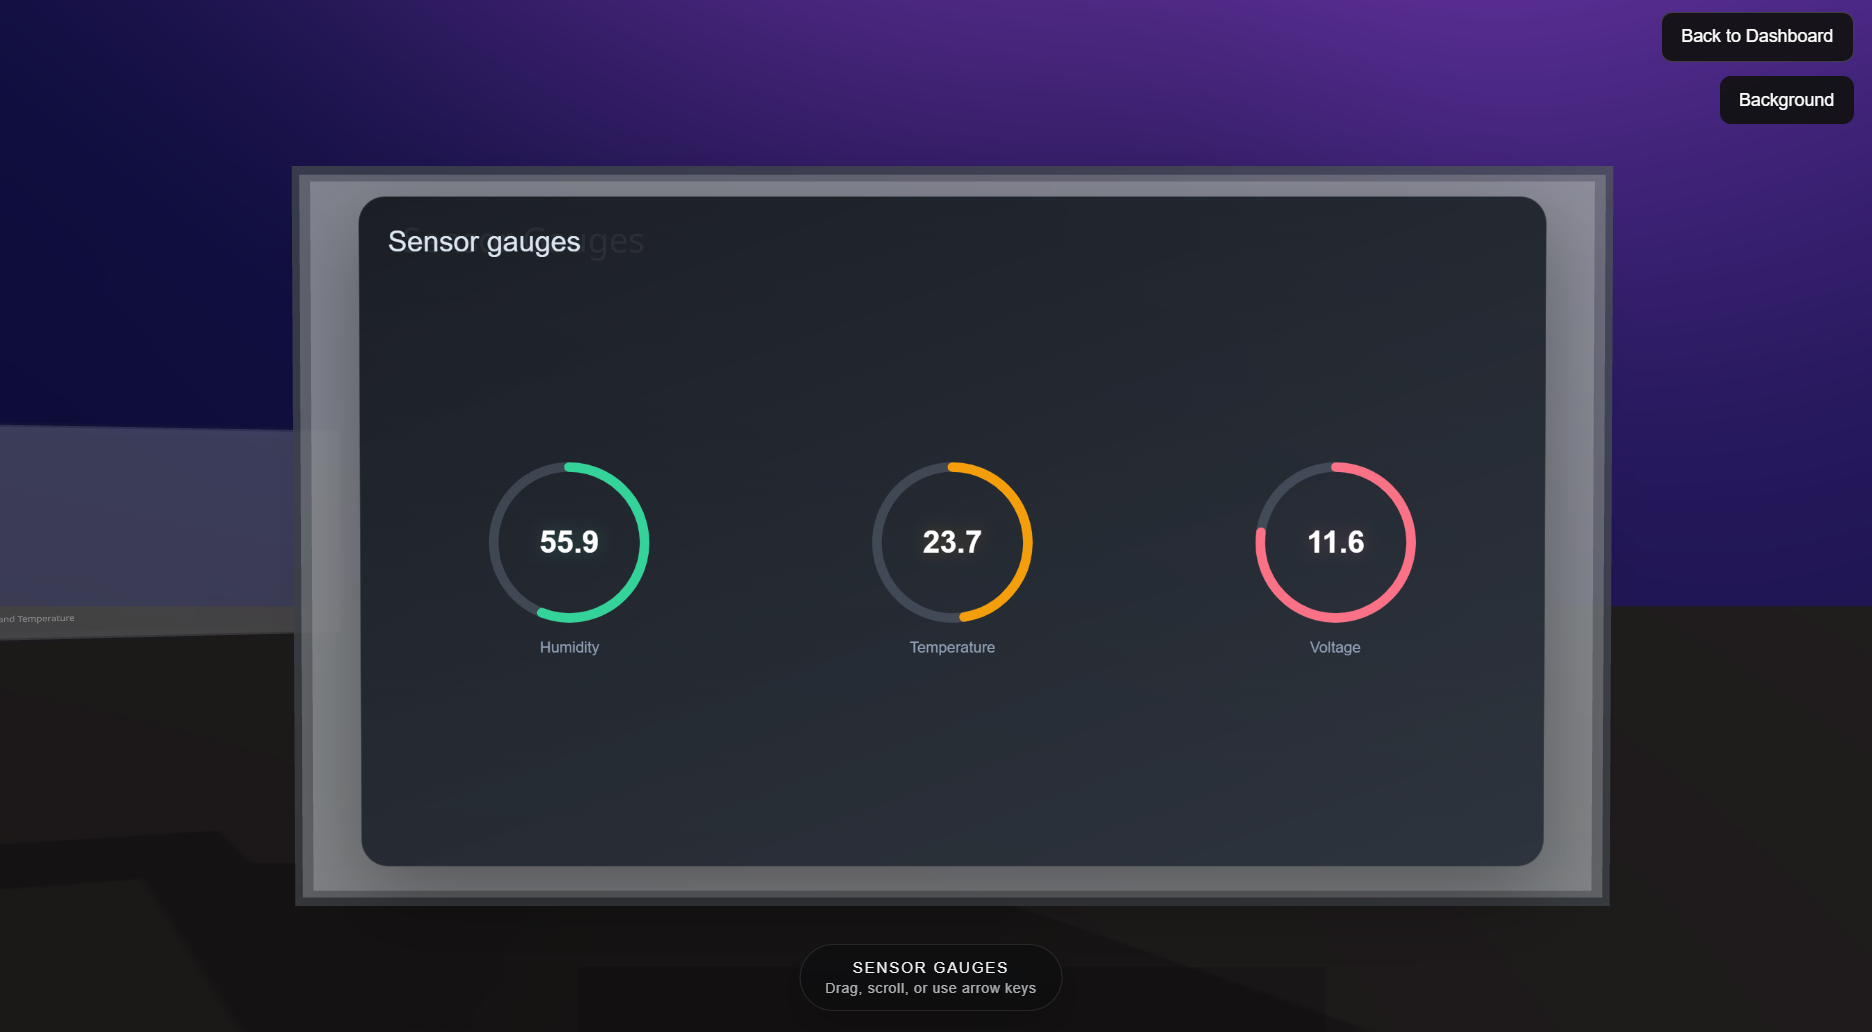
\includegraphics[width=\linewidth]{figures/sensor-gauges.png}
  \caption{Gauge-based summary view of the three principal metrics.}
  \label{fig:gauges}
\end{figure}

\subsection{Temperature-Humidity Timeline}
This panel uses a dual-axis line chart to show humidity and temperature together over time. The humidity series is rendered in green and temperature is rendered in orange. By combining both into one chart, the user can observe whether the two variables rise together, diverge, or follow different cycles. This is useful in environmental diagnostics because many changes are not meaningful in isolation.

\begin{figure}[!t]
  \centering
  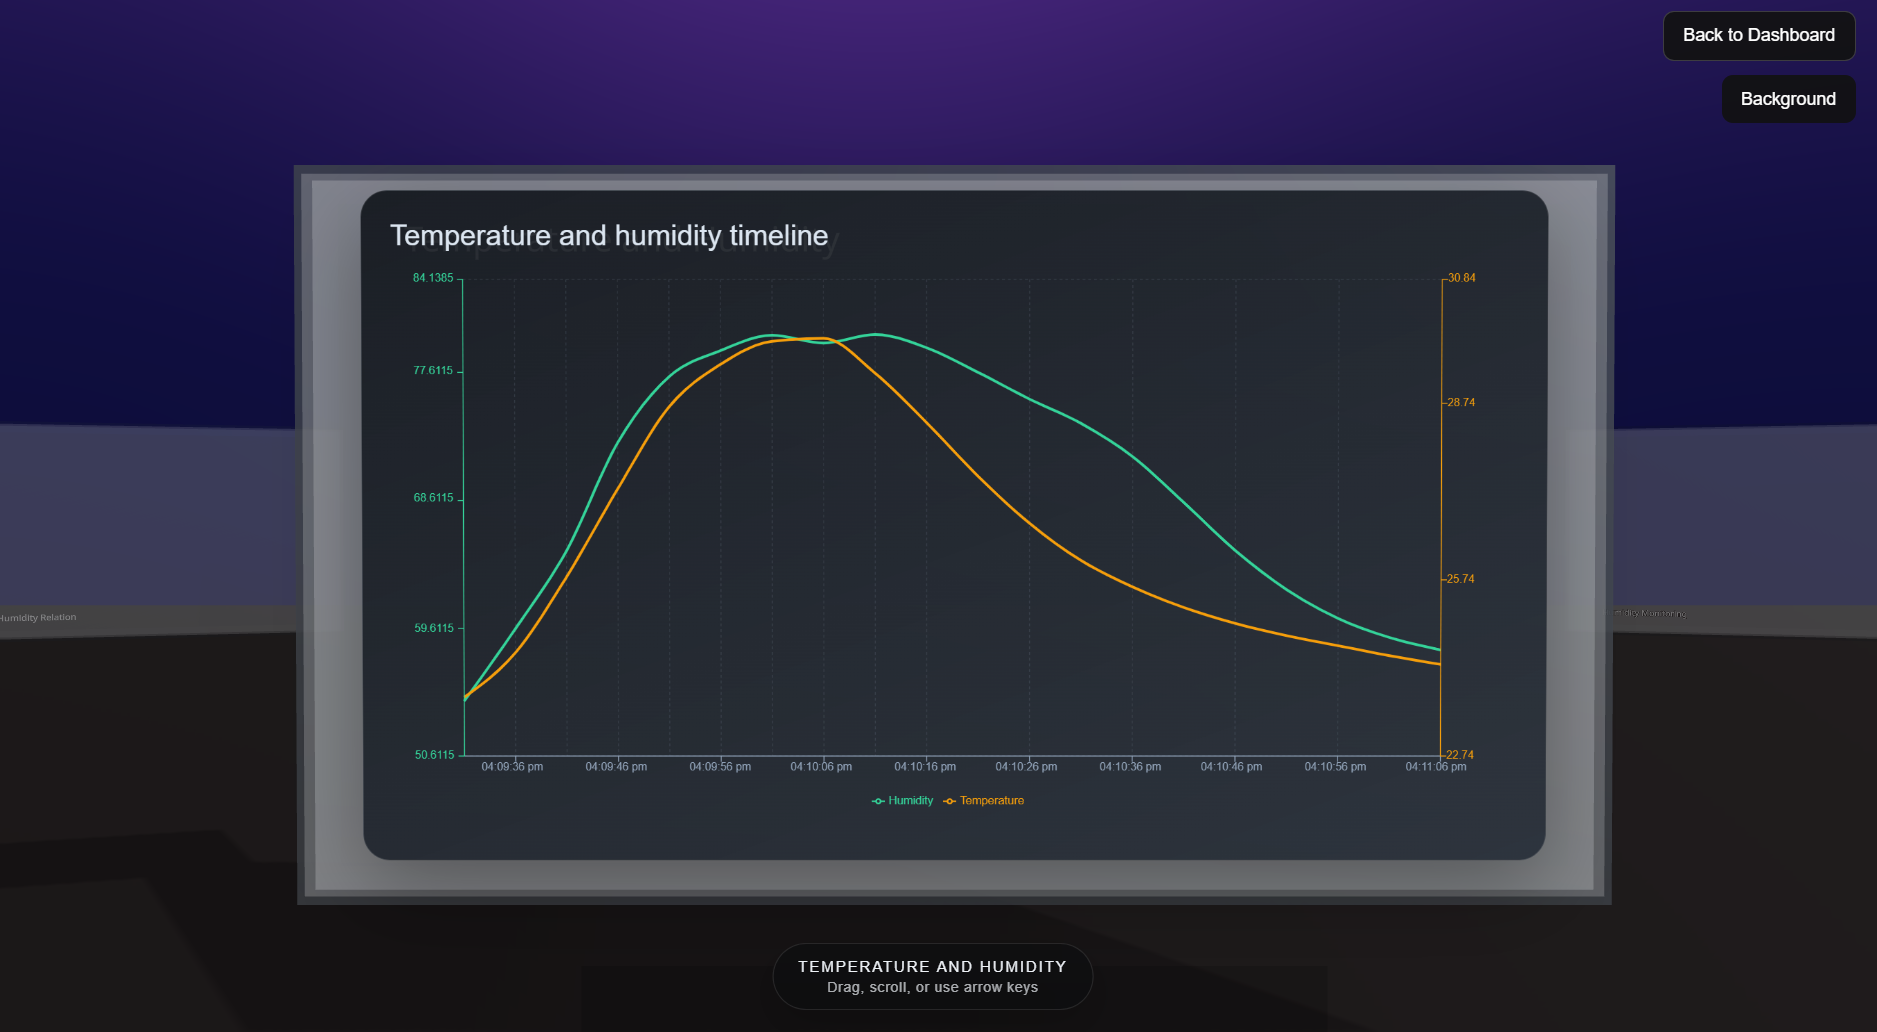
\includegraphics[width=\linewidth]{figures/temperature-humidity-timeline.png}
  \caption{Dual-axis timeline for humidity and temperature.}
  \label{fig:timeline}
\end{figure}

\subsection{Voltage-Temperature Comparison}
The voltage-temperature panel is a composed chart in which voltage is shown through bars and temperature is shown through a line. Internally, both series are normalized to percentage scales so that they can share the same chart area while still displaying readable axis labels for the original units. This design allows the user to inspect whether voltage changes correlate with thermal changes during operation.

\begin{figure}[!t]
  \centering
  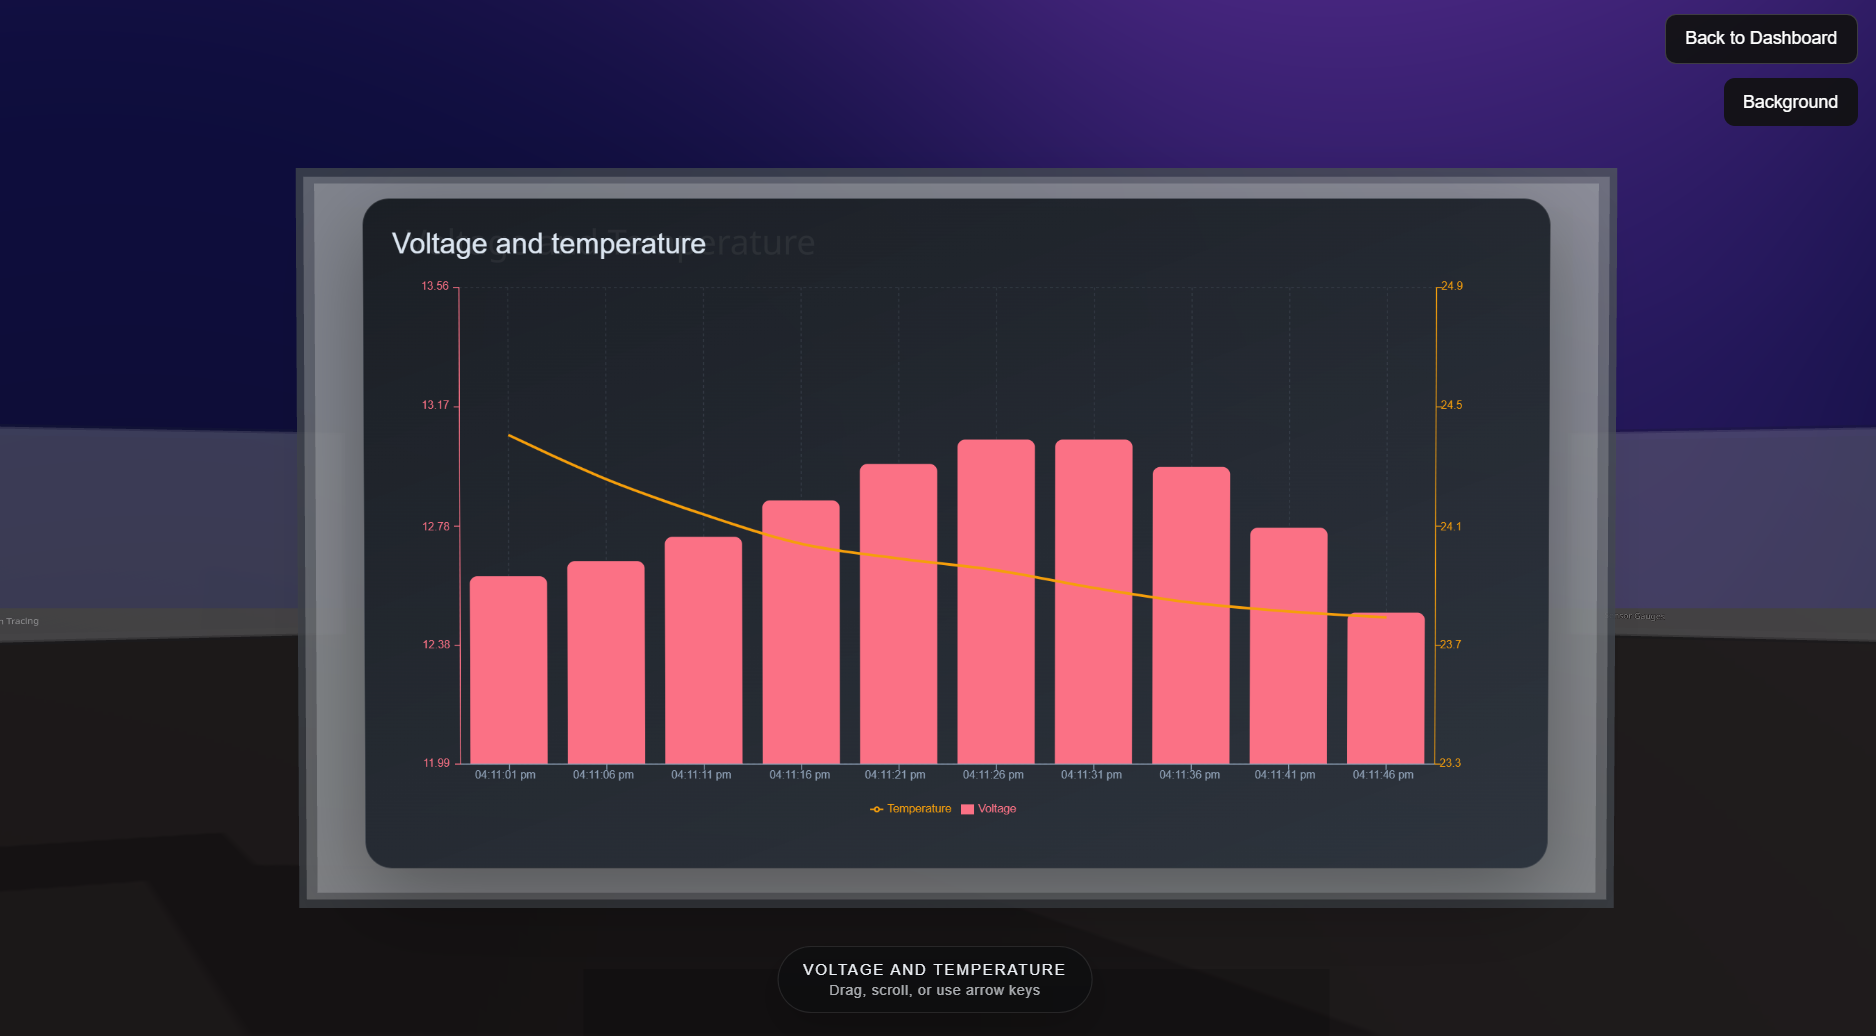
\includegraphics[width=\linewidth]{figures/voltage-temperature.png}
  \caption{Combined voltage and temperature panel used for comparative monitoring.}
  \label{fig:voltage-temp}
\end{figure}

\subsection{Location Tracing Panel}
The location tracing panel provides spatial context to the monitored asset, such as a truck or remote mobile unit. Inside the dashboard it appears as an embedded Mapbox-based preview with its own mini controls for zooming and orientation reset. When expanded, it opens a full-screen interactive map overlay with 3D buildings, satellite streets, terrain exaggeration, and a marked tracked position.

\begin{figure*}[!t]
  \centering
  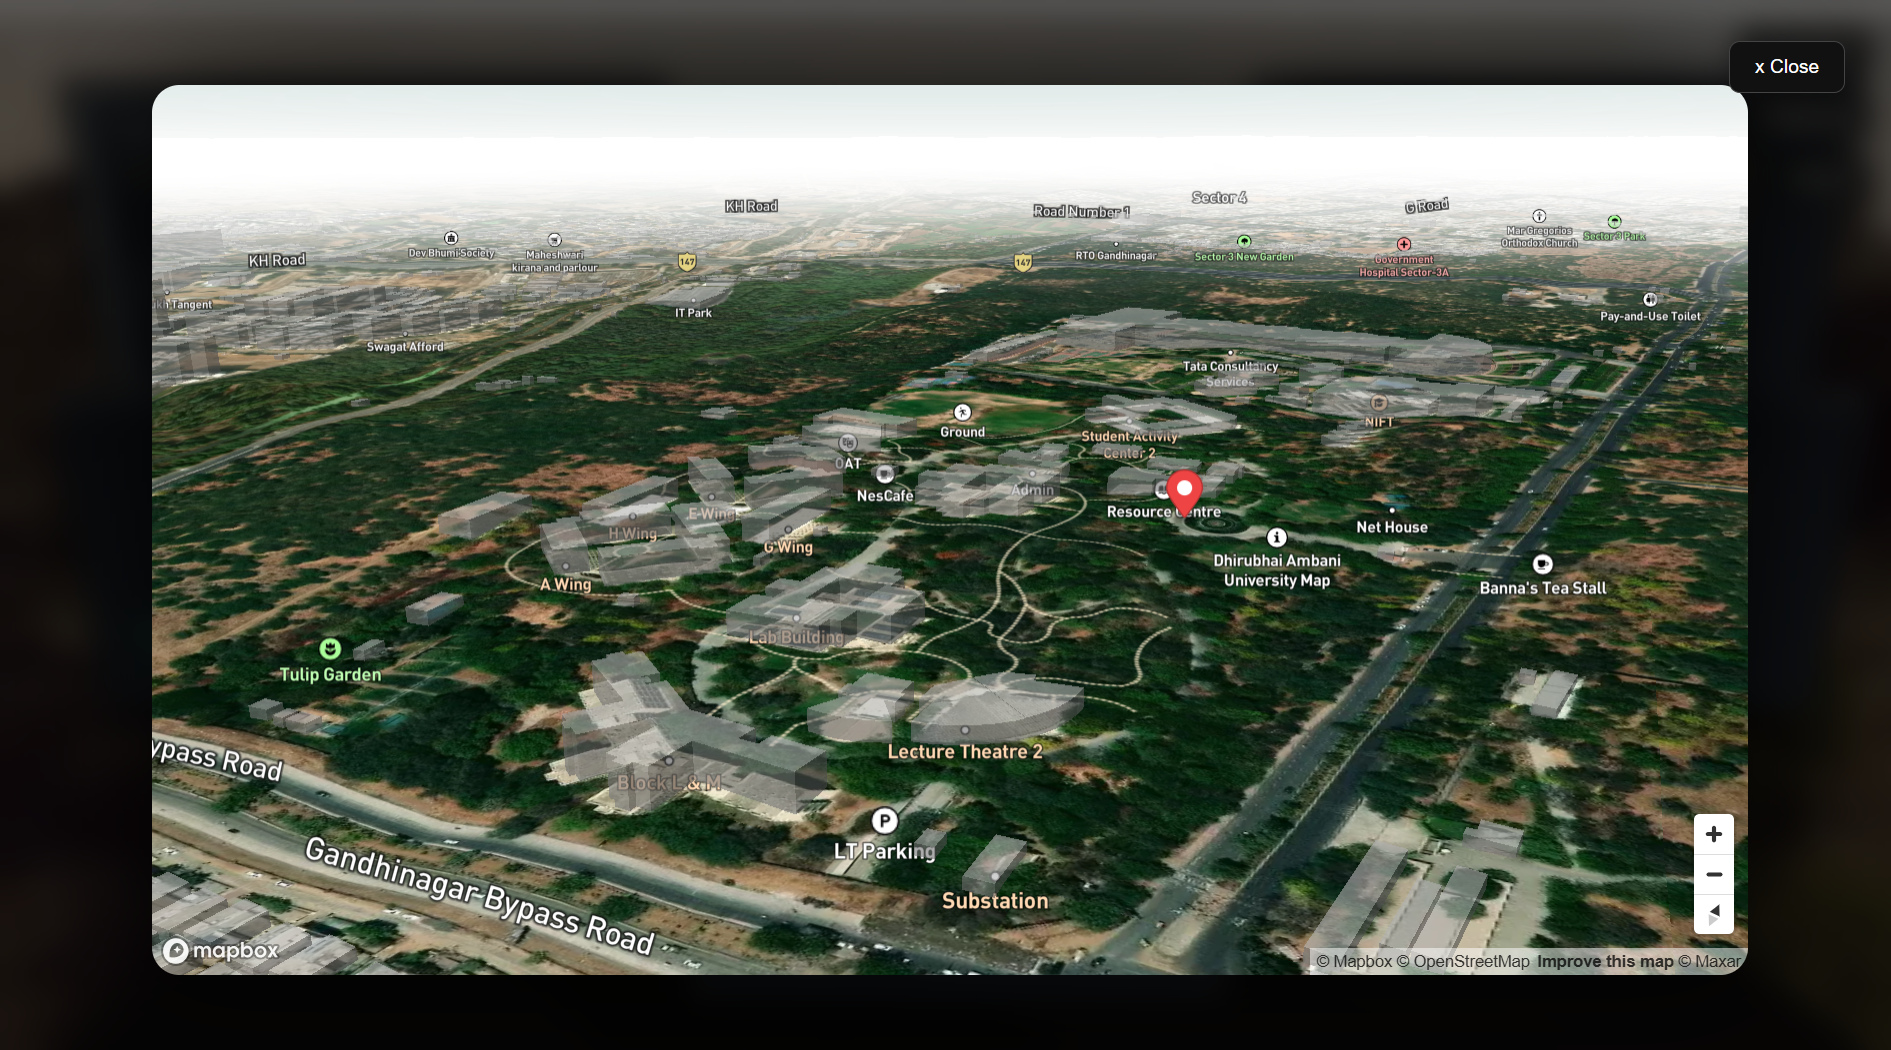
\includegraphics[width=0.9\textwidth]{figures/map-overlay.png}
  \caption{Expanded Mapbox location overlay with 3D terrain and marked asset position.}
  \label{fig:map}
\end{figure*}

\section{Interaction Modes and User Experience Design}
\subsection{Default Dashboard Mode}
In the default mode, all six panels are visible together in a spatial arrangement. The placement is intentionally distributed across left, right, top, center, and bottom positions so that the dashboard resembles a control wall instead of a flat list of charts. The user can orbit around the environment and click a panel to focus the camera on it.

\subsection{Slider Mode}
Slider mode is a focused inspection environment. Instead of showing all panels equally, it arranges them along a reel and allows the user to move through them using drag gestures, the mouse wheel, or arrow keys. Only the active panel is fully emphasized, while neighbouring panels appear as smaller hints in the background. This is particularly effective for detailed chart reading or for presentation use.

\subsection{Move Mode}
Move mode allows the user to drag the panels to new positions. This introduces personalization into the dashboard. Different operators may prefer different spatial layouts depending on which metrics they monitor most frequently. The design is therefore not rigid; it supports a user-shaped workspace.

\begin{figure}[!t]
  \centering
  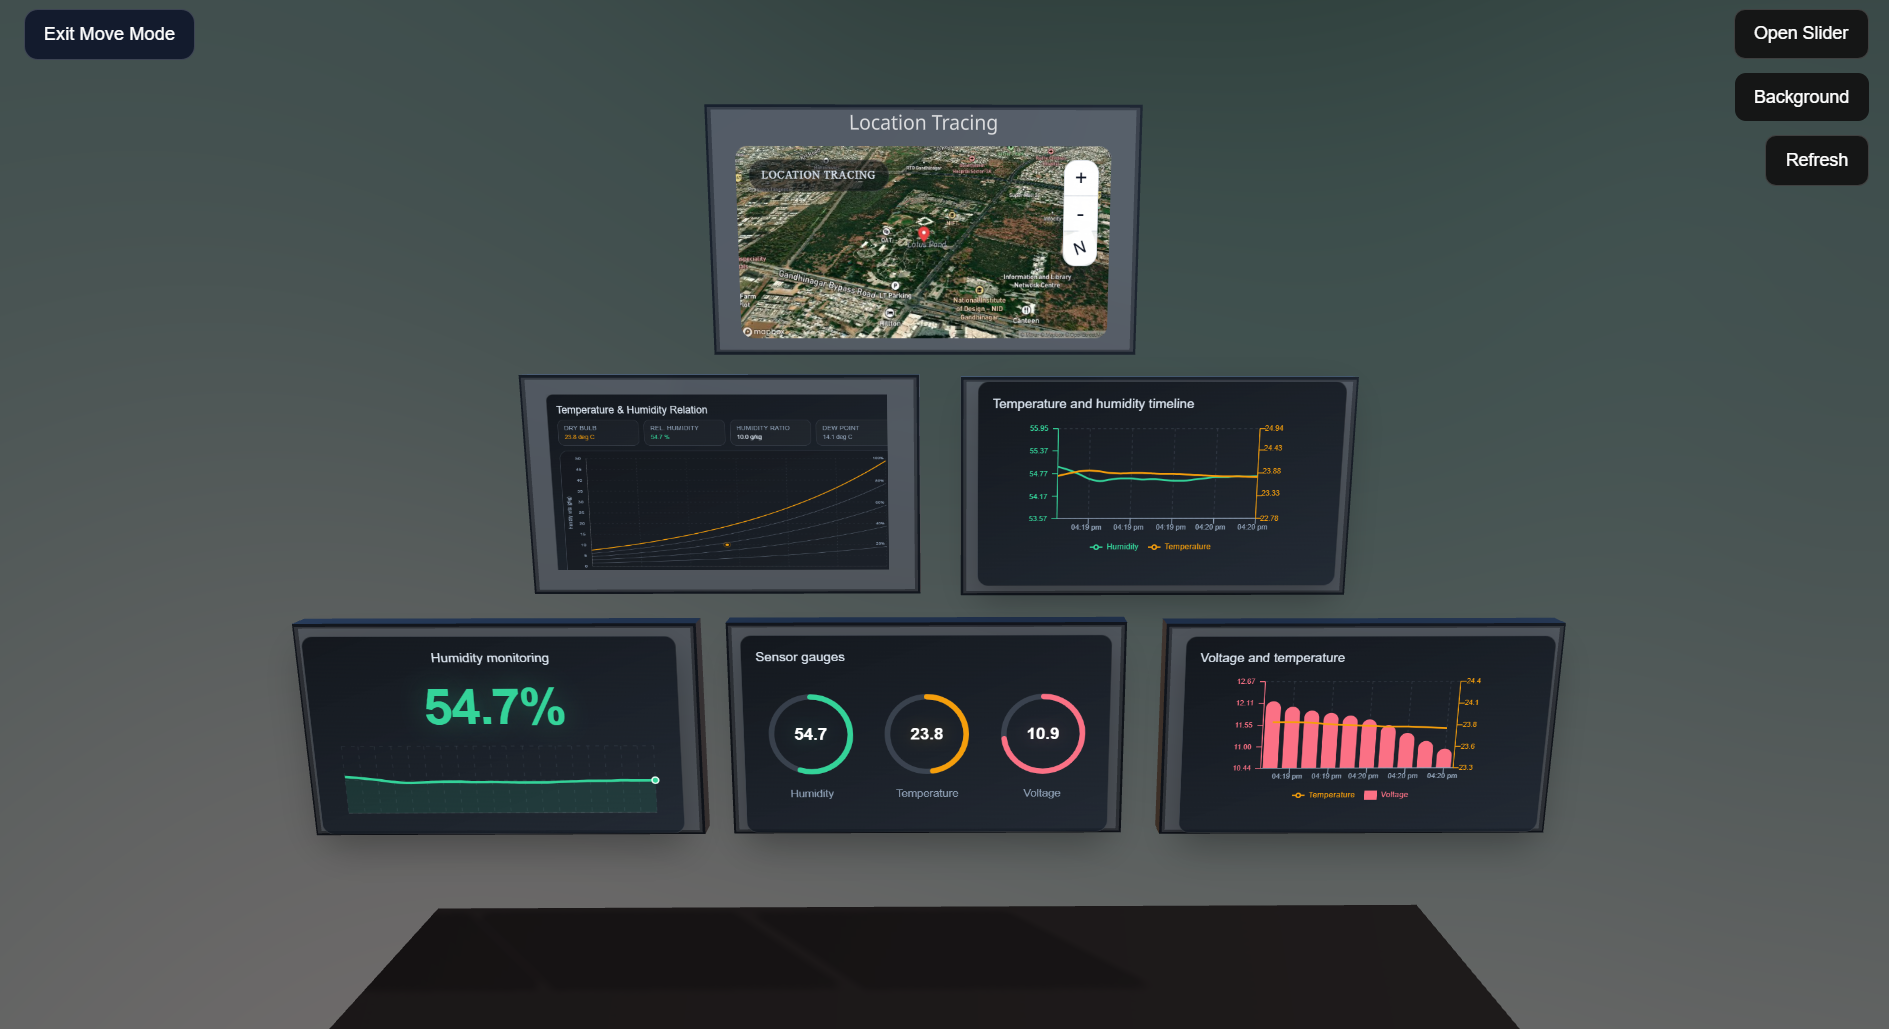
\includegraphics[width=\linewidth]{figures/move-mode.png}
  \caption{Move mode, where the user can reposition the panels to create a preferred workspace layout.}
  \label{fig:move}
\end{figure}

\subsection{Experience Mode}
Experience mode places the user at the center of the dashboard. Instead of controlling the scene from outside, the user steps into the spatial arrangement and observes the panels from within. This mode is supported by guide prompts and camera transitions that move the viewing position to a dedicated internal observation point.

\begin{figure}[!t]
  \centering
  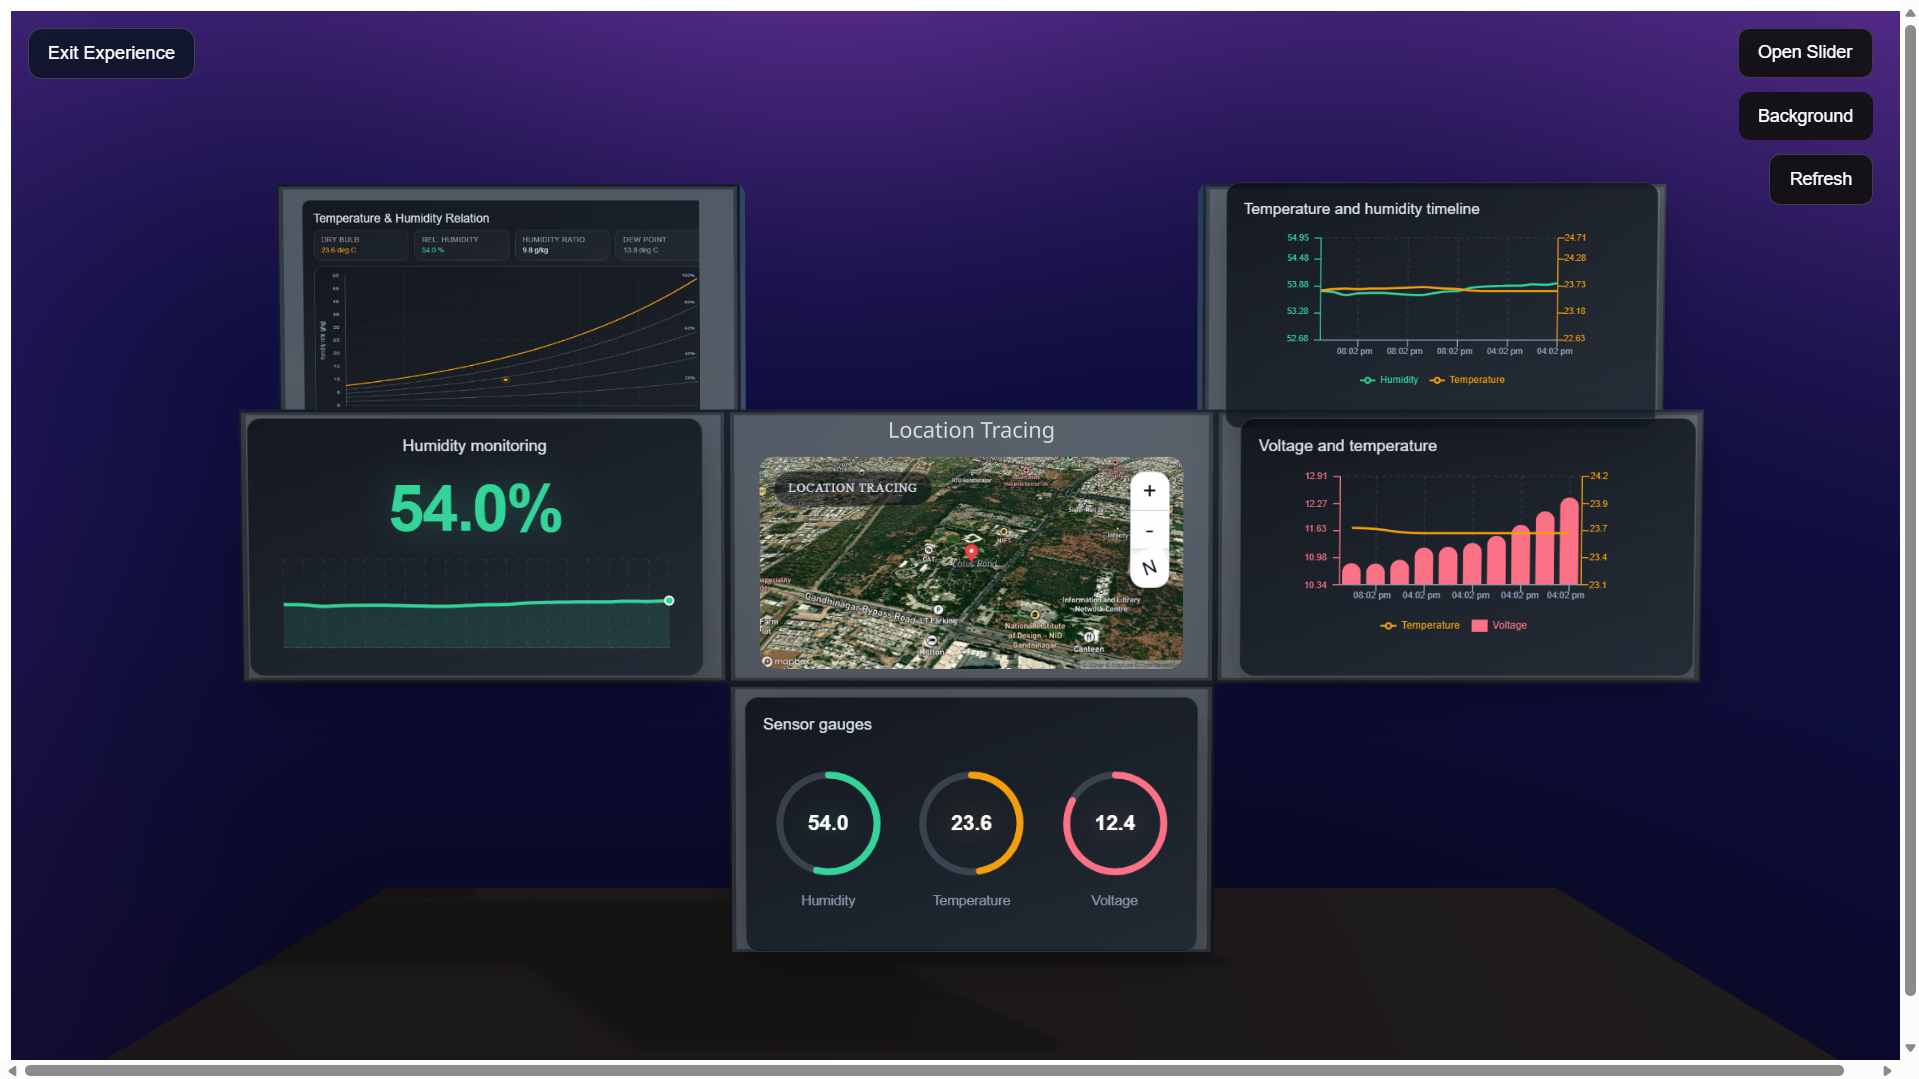
\includegraphics[width=\linewidth]{figures/experience-zone.png}
  \caption{Experience mode, in which the user stands inside the dashboard environment.}
  \label{fig:experience}
\end{figure}

\subsection{Spatial Audio Feedback}
The immersive experience is reinforced by a spatial audio subsystem. A looping audio buffer is attached to panel anchors using Three.js positional audio. Panels on the left side pan toward the left audio channel, panels on the right side pan toward the right channel, and center panels remain neutral. GSAP is used to fade audio in and out smoothly as the user hovers different panels in experience mode. This transforms the dashboard from a purely visual scene into a multimodal interface.

\subsection{Background and Atmosphere Controls}
The scene supports both HDRI environments and animated gradient backgrounds. The HDRI options create realistic lighting and reflections, while the gradient mode provides stylized presentation presets. Users can choose built-in themes or adjust the three gradient color stops manually. These preferences are saved in local storage so the scene restores the user's chosen look across sessions.

\begin{figure}[!t]
  \centering
  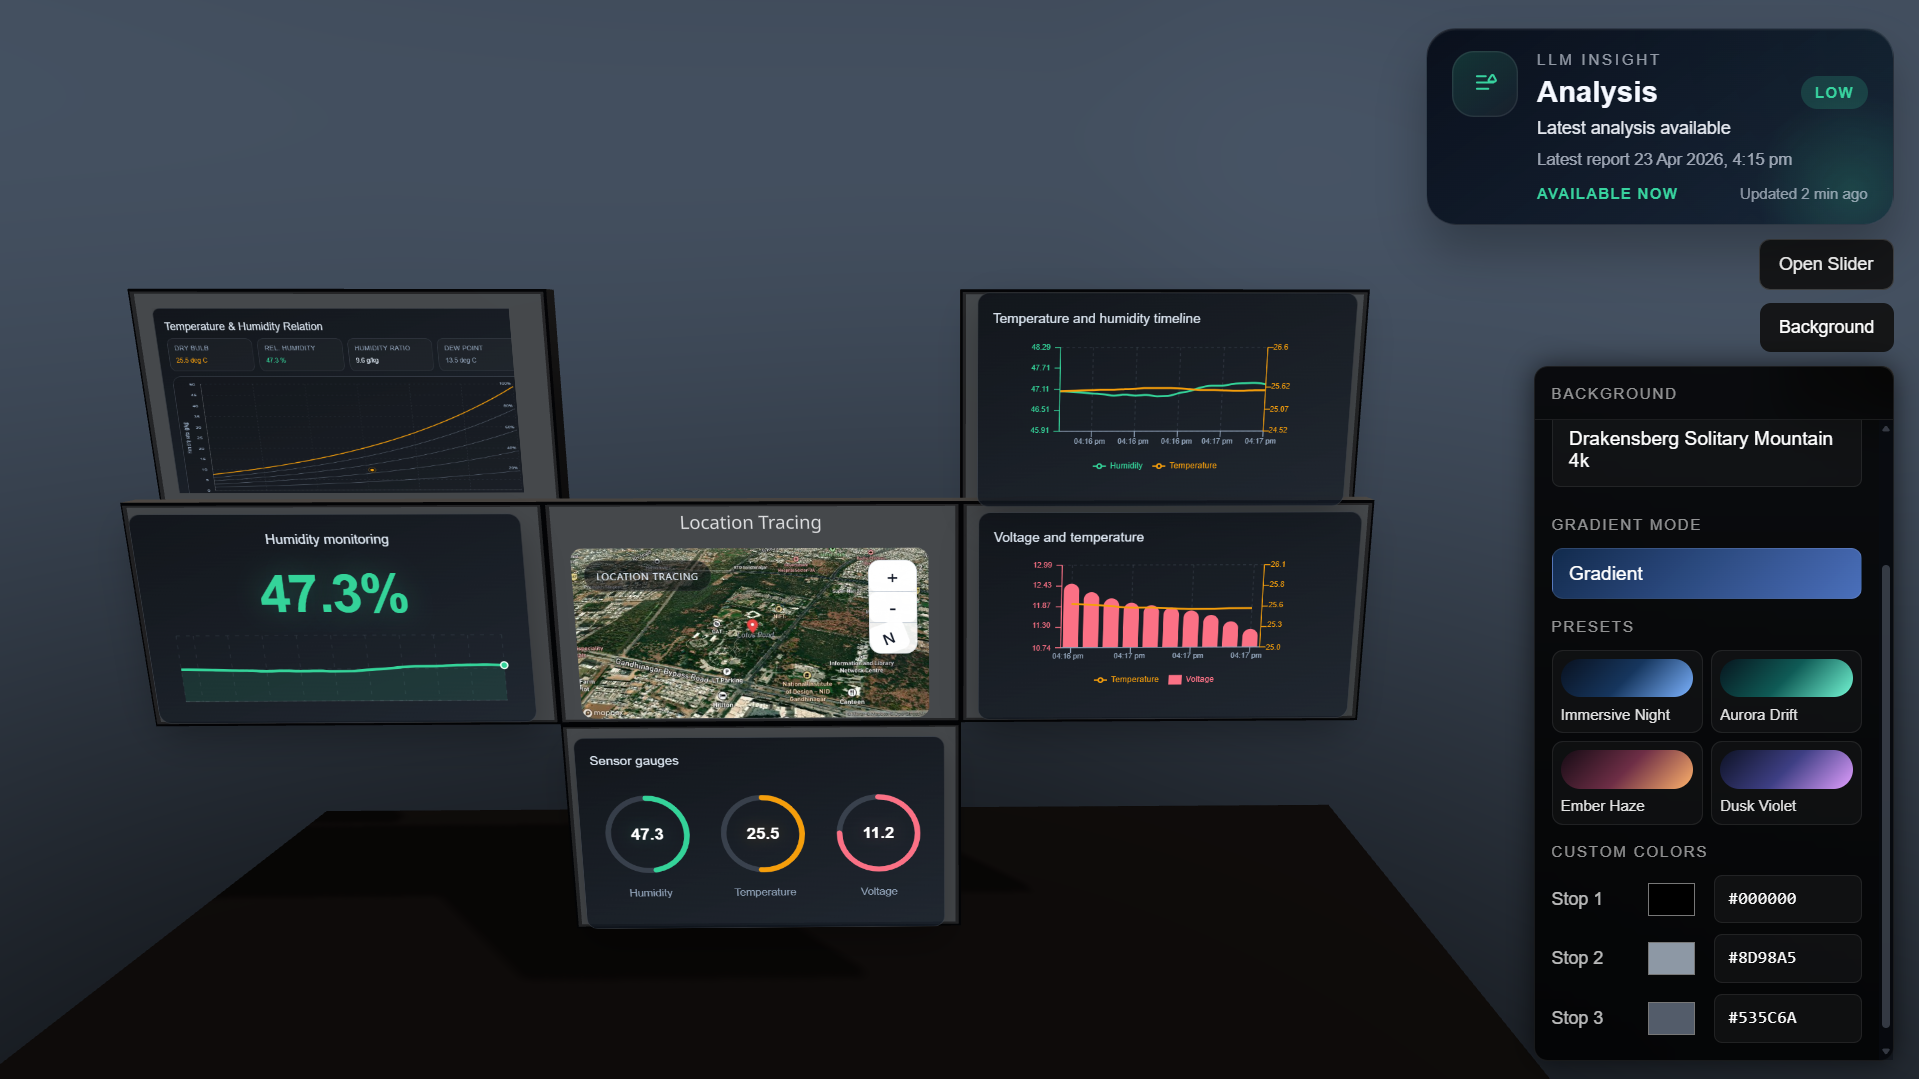
\includegraphics[width=\linewidth]{figures/background-controls.png}
  \caption{Background customization interface with HDRI presets, gradient mode, and custom color stops.}
  \label{fig:background}
\end{figure}

\section{LLM-Based Analysis Module}
The analysis subsystem adds a semantic layer on top of the raw charts. Instead of requiring the operator to manually infer the situation from the graph patterns, the dashboard can fetch a processed analysis report from the backend and present it in natural language.

\subsection{Analysis Window and Statistical Summary}
Before the LLM is invoked, the Raspberry Pi backend reads the most recent 5-minute time window of sensor records and computes descriptive statistics for each measured variable. For temperature, humidity, pressure, and gas resistance, the backend derives minimum, maximum, average, starting value, ending value, delta, and population standard deviation where applicable. These derived values are used to build a compact environmental summary for interpretation.

\subsection{Rule-Based Flag Detection}
In addition to descriptive statistics, the backend performs rule-based flag detection. Examples include low sample count, significant temperature change, high temperature, unstable temperature, high humidity, low humidity, significant pressure change, and substantial gas-resistance drop. These flags act as machine-readable cues for the local LLM and also remain useful for debugging.

\subsection{Local Ollama Integration}
The LLM module is implemented through Ollama running locally at \texttt{http://localhost:11434/api/generate}. The configured model is \texttt{qwen2.5:0.5b}. The prompt explicitly instructs the model to behave as a local environmental monitoring assistant and to use only the supplied sensor summary and flags. It also forbids overclaiming, for example by warning the model not to invent exact VOC ppm values, AQI values, CO$_2$ concentration, smoke concentration, or specific gas identity from raw BME680 gas resistance alone.

The analysis payload is normalized into the following fields:
\begin{itemize}
\item timestamp of analysis generation,
\item situation label,
\item threat level,
\item alert list,
\item detailed narrative analysis,
\item recommended action,
\item optional summary,
\item optional structured flags.
\end{itemize}

The Ollama request is made with a strict JSON schema so that only these fields are returned. This structured-output design is important because it converts a general-purpose language model into a predictable subsystem that the frontend can render safely.

\subsection{Fallback and Failure Handling}
The backend contains a clear fallback strategy for failure conditions. If Ollama is unavailable, times out, returns empty text, or responds with invalid JSON, the system still emits a valid analysis object. In such cases the dashboard reports that sensor collection is active but local LLM analysis failed, and it recommends checking whether Ollama is running and whether the model is available.

The application checks this feed every five minutes by default and also allows user-triggered refresh. A compact action card on the dashboard shows the latest availability, last update time, and a threat-tone badge. When opened, the full drawer presents the entire report in a structured form. If analysis is temporarily unavailable, the interface degrades gracefully by showing loading states, empty states, or stale-data warnings instead of failing silently.

This design is significant because it converts the dashboard from a passive visualization tool into an active decision-support interface. The operator does not merely see numbers; the system explains what those numbers may mean operationally.

\section{Ease of Use}
Ease of use was an explicit design priority in the project. Several implementation choices contribute to this goal.

\subsection{Readable Information Hierarchy}
Each panel has a clear visual purpose. Large typography is used for headline values, and detailed charts are reserved for focused panels. This reduces the cognitive load on first glance.

\subsection{Multiple Access Patterns}
Different users interact with data differently. Some prefer a full overview, some need a single chart in isolation, and some benefit from a more immersive experience. By providing dashboard mode, slider mode, and experience mode, the system supports all three interaction styles without duplicating data logic.

\subsection{Graceful Failure Behaviour}
The interface does not assume a perfect environment. If streaming is unavailable, fallback polling continues. If the map token is missing, the preview explains that configuration is required. If analysis fails, the panel still remains usable and explains the error state. Such behaviours make the system more practical outside ideal demonstration conditions.

\subsection{Persistent User Preferences}
Background settings and cached history are stored locally. This reduces repetitive setup effort and allows the application to feel more continuous and personalized.

\section{Implementation Details of Important Modules}
\subsection{Panel Definition Strategy}
All dashboard panels are described through a central definition list that stores panel keys, default positions, whether they are movable, and the label used in slider mode. This makes the layout easy to extend. New panels can be added by inserting another definition and mapping it to a content component.

\subsection{Panel Content Strategy}
The \texttt{useControlPanels} hook acts as an adapter between raw chart data and rendered panels. For each panel key it selects the appropriate component, passes the relevant values, and adjusts its rendering behaviour based on whether the current scene is the dashboard or the slider reel.

\subsection{Map Rendering Strategy}
The embedded map uses a static map image for performance inside the dashboard panels. When the user requests more detail, the application opens a full interactive overlay using Mapbox GL. This two-level approach is efficient because it avoids heavy interactive rendering for every frame of the main scene while still providing a rich map experience when needed.

\subsection{Camera Behaviour}
Camera motion is not abrupt. The dashboard uses interpolated transitions for panel focus, entering experience mode, and returning home. This improves comfort and makes navigation feel deliberate rather than mechanical.

\subsection{Edge-Backend Reliability Strategy}
The Raspberry Pi server is designed for long-running operation. It maintains in-memory latest snapshots for fast API responses, stores persistent JSON files for recovery after restart, and reloads the most recent saved analysis at startup. This means the dashboard can resume with meaningful context even after the backend process restarts.

\section{Learning Outcomes}
The project led to the development of both technical and non-technical skills.

\subsection{Technical Learning Outcomes}
\begin{itemize}
\item Learned how to configure and read a BME680 sensor on Raspberry Pi 5 for continuous environmental monitoring.
\item Understood how to design a lightweight edge backend using Flask, Flask-SocketIO, JSONL logging, and file-lock-based concurrency safety.
\item Learned how to build immersive browser-based 3D applications using Three.js, React Three Fiber, and React Three XR.
\item Understood how to synchronize REST APIs, Socket.IO streaming, and local caching within one frontend data pipeline.
\item Gained hands-on experience with designing reusable React hooks for independent application subsystems.
\item Implemented mixed visual analytics using line charts, bar charts, gauges, and a psychrometric-style derived plot.
\item Learned to integrate Mapbox previews and interactive terrain-enabled location overlays.
\item Understood how to attach positional audio to scene objects and control it through hover-driven interaction.
\item Learned how to normalize backend data and make a visualization system resilient to incomplete or delayed sensor feeds.
\item Explored how a locally hosted Ollama model with structured JSON output can be embedded into a live monitoring workflow.
\end{itemize}

\subsection{Non-Technical Learning Outcomes}
\begin{itemize}
\item Improved interface planning by thinking about operator comfort and not only technical correctness.
\item Strengthened debugging and iteration skills while integrating multiple libraries in one application.
\item Improved system-level thinking by balancing performance, usability, immersion, and reliability.
\item Learned to communicate technical insights through both visual design and structured report writing.
\end{itemize}

\section{Contributions}
The project required contributions across UI design, data engineering, visualization, and interaction design.

\subsection{Technical Contributions}
\begin{itemize}
\item Implemented Raspberry Pi 5 based sensor acquisition using the BME680 environmental sensor.
\item Built a Flask and Flask-SocketIO backend that serves current readings, historical readings, and analysis output.
\item Designed a safe JSONL logging and cleanup workflow using file locks and rolling retention.
\item Developed a React and WebXR-based 3D dashboard architecture for sensor monitoring.
\item Implemented reusable scene components, panel wrappers, and chart modules for the immersive interface.
\item Built a hybrid data pipeline combining historical fetch, live streaming, fallback polling, and local caching.
\item Implemented the psychrometric-style environmental relation panel using derived calculations for humidity ratio and dew point.
\item Developed slider mode, move mode, and experience mode to support multiple interaction styles.
\item Integrated spatial audio feedback into the experience zone using Three.js audio and GSAP transitions.
\item Built a Mapbox-based location module with both embedded preview and full-screen overlay modes.
\item Integrated a local Ollama-based LLM pipeline that consumes summary statistics and flags and returns structured environmental interpretation.
\item Integrated and normalized the analysis feed into a compact action card and a detailed report drawer.
\item Added persistent background customization with HDRI and gradient scene themes.
\end{itemize}

\subsection{Non-Technical Contributions}
\begin{itemize}
\item Designed the interface flow so that novice users can still interpret the dashboard without reading implementation details.
\item Structured the project in a modular way so that future contributors can replace placeholder data sources with real hardware feeds.
\item Prepared documentation and explanatory material to make the system presentable as an academic project.
\end{itemize}

\section{Limitations and Future Scope}
Although the current implementation is already feature-rich, several improvements can further strengthen the system:
\begin{itemize}
\item replace the current frontend-generated voltage signal with a true battery voltage sensor feed,
\item add pressure and gas resistance panels, since those values are already normalized in the frontend,
\item store panel positions persistently after move mode so that personalized layouts survive refresh,
\item integrate anomaly detection or forecasting models in addition to descriptive LLM analysis,
\item extend the WebXR pathway to support dedicated AR or VR hardware sessions more deeply,
\item add authentication, multi-device monitoring, and backend-side historical analytics for production deployment.
\end{itemize}

\section{Conclusion}
This project demonstrates how a monitoring interface can evolve from a flat dashboard into an immersive decision-support environment. By combining React-based application structure, Three.js-powered 3D rendering, WebXR-ready scene management, chart-driven analytics, Mapbox geographic context, real-time sensor updates, spatial audio, and LLM-generated analysis, the system creates a more expressive and intuitive way to understand environmental and battery conditions.

The resulting platform is not only visually distinctive but also architecturally meaningful. It shows how modern frontend technologies can be used to convert raw IoT readings into an environment that supports observation, exploration, personalization, and action. With real battery voltage integration and further backend expansion, the system can develop from a strong academic prototype into a practical monitoring solution for industrial and field applications.

\balance
\end{document}
